%!TEX root = ../dokumentation.tex
\chapter{Theoretischer Hintergrund}
In diesem Kapitel wird der theoretische Hintergrund im Zusammenhang mit den in dieser Arbeit erwähnten Themen erläutert. Hierbei werden unter anderem verschiedene Ansätze der Modifizierung des Innovationsprozesses wie Open Innovation, Crowdsourcing sowie Crowdfunding vorgestellt. Darüber hinaus werden die Unterschiede zwischen Crowdfunding und Corporate Crowdfunding klargestellt.
\section{Open Innovation}
Open Innovation beschreibt den Innovationsprozess, der nicht innerhalb eines Unternehmens seine Grenzen hat, sondern Akteure unabhängig von deren institutioneller Zugehörigkeit als Ideengeber, Konzeptentwickler oder auch Innovationsumsetzer in die Gestaltung von Innovationen einbindet \cite[85]{Zerfaß2009}. Bei der Öffnung des Innovationsprozesses treten dabei drei zentrale Akteure in Erscheinung.

\begin{table}[htb]
\centering
\begin{tabular}{p{4cm} | p{5cm} | p{4.8cm}}
\hline
\textbf{Innovatorengruppe} & \textbf{Herkunft} & \textbf{Quellen} \\
\hline
Kerninnovatoren im Unternehmen & Mitarbeiter der Abteilungen Forschung \& Entwicklung und Strategische Innovation & \citeauthor{schumpeter1934} \citeyear{schumpeter1934}; \newline
	\citeauthor{wheelwright1992} \citeyear{wheelwright1992};  \newline
	\citeauthor{vissers_dankbaar2002} \citeyear{vissers_dankbaar2002} \\ 
\hline
Periphere Innovatoren im Unternehmen & Mitarbeiter in der Breite des Unternehmens & \citeauthor{Robinson:1486035} \citeyear{Robinson:1486035}; \newline
	\citeauthor{berger2005} \citeyear{berger2005}; \newline
	\citeauthor{Huff2006} \citeyear{Huff2006}; \\
\hline
Externe Innovatoren & Kunden, Lieferanten, Wertschöpfungspartner, Universitäten, Forschungsinstitutionen & \citeauthor{Hippel1978} \citeyear{Hippel1978}, \citeyear{Hippel1986}, \citeyear{Hippel2006}; \citeauthor{reichwald2006open} \citeyear{reichwald2006open}; \\
\hline
\end{tabular}
\caption{Akteure der Open Innovation \cites[91]{Zerfaß2009}[8]{moslein2010open} }
\end{table}

Bei der Betrachtung der heutigen Leistungspaletten vieler Unternehmen fällt in der Regel auf, dass der Großteil von Produkten den Kerninnovatoren im Unternehmen zuzuschreiben sind. Unterstützend zum Entwicklergeist der Kerninnovatoren werden bei der Open Innovation jedoch vermehrt externe Innovatoren in Form von Kunden, Lieferanten und Wertschöpfungspartnern dazu aufgerufen, ihre Ideen in den Innovationsprozess mit einfließen zu lassen. Ein wesentlicher Grund hierfür sind die verschiedenen Interessen der einzelnen Geschäftspartner. Fällt zum Beispiel einem Kunden während der Nutzung eines Produktes auf, dass er das ein oder andere Feature vermisst, kann er dies in den weiteren Innovationsprozess einfließen lassen, um somit die anstehende Iteration des Produktlebenszyklus zu verbessern. Zusätzlich zu den externen Innovatoren zielt Open Innovation auch darauf ab, periphere Innovatoren in die Gesamtinnovationsstrategie einzubeziehen \cite[91\psq]{Zerfaß2009}.

\section{Crowdfunding}
Crowdfunding stellt neben Open Innovation eine weitere innovative Möglichkeit der Kapitalbeschaffung dar, welche die Finanzierung eines Projekts durch eine Vielzahl kleinerer Investoren als Ziel sieht \cite[59\psq]{Himmer2019}. Für die Umsetzung wird dabei generell auf darauf spezialisierte Plattformen zurückgegriffen \cite{Sixt2014}. Zum Einstieg in dieses Thema soll die verbreitete Definition des Crowdfundings von \citeauthor{ordani} als präzise Umschreibung des Finanzierungsphänomens dienen: 

\begin{quote}
	\glqq Crowdfunding is a collective effort by people who network and pool their money together, usually via the Internet, in order to invest in and support efforts initiated by other people or organizations \cite{ordani}.\grqq{}
\end{quote}

\subsection{Crowdfunding Akteure}
Bei der Betrachtung des Crowdfunding Prozesses wird überwiegend von drei verschiedenen Akteuren gesprochen. Hierzu gehören die Kapitalnehmer, die Intermediäre sowie die Kapitalgeber, welche in Abbildung \ref{fig:crowdfunding_actors} genauer abgebildet sind. 

\begin{figure}[htb]
	\centering
	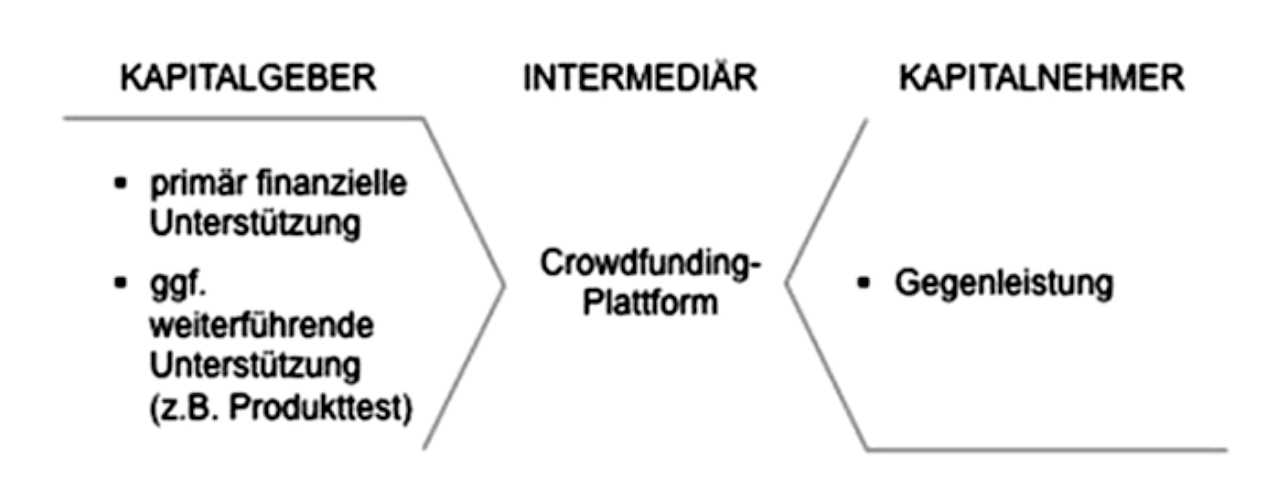
\includegraphics[width=\textwidth]{images/crowdfunding_akteure}
	\caption{Akteure des Crowdfunding-Prozesses. (Quelle: \citeauthor{Guenther2019} \citeyear{Guenther2019})}
	\label{fig:crowdfunding_actors}
\end{figure} 

Der Intermediär bietet für Kapitalnehmer und -geber eine Plattform, auf der mittels eines standardisierten Verfahrens eine Durchführung von Finanztransaktionen gewährleistet wird und ein Informationsaustausch zwischen beiden Parteien hergestellt werden kann \cites[7\psq]{Guenther2019}{moritz2015}.

\subsubsection*{Kapitelnehmer}
Kapitalnehmer, welche im vorliegenden Kontext auch als Projektinitiatoren bezeichnet werden \cite[11]{Gierczak2016}, sind sowohl Einzelpersonen als auch Unternehmen in der Früh- und Spätphase der Geschäftstätigkeit \cites{Gierczak2016}{Schwienbacher2010}[8]{Guenther2019}. Die wichtigste Anforderung aufseiten der Kapitalnehmer ist die überzeugende Darstellung des zu finanzierenden Vorhabens \cites{Guenther2019}{bouncken}. 
\subsubsection*{Intermediär (Plattform)}
Der Intermediär wird als Vermittler des Finanzierungsprozesses angesehen. Dieser stellt dabei standardisierte Prozesse zur Durchführung der Crowdfunding-Kampagnen bereit \cite[9]{Guenther2019}. Die erfolgreiche Kommunikation zwischen Kapitalgeber und -nehmer ist dabei wichtig, um eine Crowdfunding-Kampagne durchzuführen. Seitens der Intermediäre werden diesbezüglich unterschiedliche Transaktionsmechanismen angeboten \cite[9]{Guenther2019}:

\begin{itemize}
	\item ''All-or-Nothing''\newline
	Im Mittelpunkt der meisten Crowdfunding-Plattformen steht das All-or-Nothing Prinzip \cite{cumming_leboeuf_schwienbacher_2014}. Nach diesem Prinzip erhalten Projektinitiatoren den gesammelten Betrag nur dann ausbezahlt, wenn sie ihr vordefiniertes Finanzierungsziel erreichen. Dies beruht auf der Annahme, dass Geldgeber nur dann in der Lage sind ihr Projekt zu verwirklichen und die versprochenen Erträge zu erzielen, wenn sie über die dafür erforderlichen Ressourcen verfügen \cite{Gerber2011Crowdfunding}.
	\item ''Keep-What-You-Get''\newline
	Ein weiterer Transaktionsmechanismus ist das Keep-What-You-Get Prinzip, bei dem die Projektinitiatoren jede gesammelte Summe erhalten \cite{Gerber2011Crowdfunding}.  Dieses Finanzierungsprinzip wird insbesondere bei gemeinnützigen Projekten oder bei Projekten angewandt, die Crowdfunding als untergeordnete Finanzierungsquelle nutzen \cite[42\psqq]{Gebert2013}.
\end{itemize}

\subsubsection*{Kapitalgeber (Crowd)}
Kapitalgeber sind die Geldgeber auf den Crowdfunding-Plattformen. Entscheidet sich ein Kapitalgeber für die Unterstützung eines Projekts, kann er über den Intermediär eine Zahlung mittels eines Zahlungsdienstleisters tätigen. Bei solchen Transaktionen bleiben die Kapitalgeber und ihre finanziellen Beiträge zueinander anonym \cite[10]{Guenther2019}.

\subsection{Ausgestaltungsarten des Crowdfunding}
In den letzten Jahren sind eine Vielzahl verschiedenster Crowdfunding Finanzierungsmethoden aus dem Boden emporgewachsen. \citeauthor{Guenther2019} bezeichnet die folgenden Modelle als die vier Grundformen des Crowdfundings, wobei sich die finanziellen Modelle im Kern in Fremd- und Eigenkapitalfinanzierungen unterscheiden lassen.
\subsubsection*{Fremdkapitalbasiertes (lending-based) Crowdfunding}
Unter dem fremdkapitalbasierten Crowdfunding bzw. Crowdlending wird im deutschen Rechtskreis ein auf Darlehen aufbauendes Finanzierungsmodell verstanden \cite[11]{Guenther2019}. Dabei wird, beim Erreichen des Finanzierungsziels, ein Kreditvertrag zwischen Kreditnehmer und Kreditgebern abgeschlossen. Eine generelle Abbildung des Ablaufs ist in Anhang \ref{sec:A} zu finden.
\subsubsection*{Eigenkapitalbasiertes (equity-based) Crowdfunding}
Beim eigenkapitalbasierten Crowdfunding bzw. Crowdinvesting, investiert die Crowd in Form von Eigen- oder Mezzanine\footnote{Mischform zwischen Eigen- und Fremdkapital \cite{Schrecker2012}}-Kapital in den Kapitalnehmer. Im Gegenzug erhält der Investor Anteile, eine Gewinnbeteiligung oder anderweitig variable Vergütungen \cites[13]{Guenther2019}[195\psq]{Looy2015}. Kurz gefasst handelt es sich in diesem Sinne um eine Beteiligungsfinanzierung.
\subsubsection*{Spendenbasiertes (donation-based) Crowdfunding}
Das spendenbasierte Crowdfunding ist eines der nicht-finanziellen Crowdfunding Modelle. Der Investor, welcher für seine Spende keine Gegenleistung erhält, erfüllt infolgedessen lediglich einen ideellen Zweck. Aus rechtlicher Sicht ist dieses Modell als am wenigsten aufwendig anzusehen, da es auf einer Schenkung basiert. \cite[15\psq]{Guenther2019}
\subsubsection*{Belohnungsbasiertes (reward-based) Crowdfunding}
Eines der ältesten und einfachsten Wege in Crowdfunding-Projekte zu investieren, ist das belohnungsbasierte Crowdfunding, bei welchem der Investor eine vordefinierte Belohnung für sein Investment erhält. Diese Belohnungen sind meist im Umfang eines T-Shirts oder einer ähnlichen Anerkennung. % WTF Grammatik??
 Bei diesem Modell liegt der Schwerpunkt nicht auf dem Erwirtschaften von Gewinnen durch Investments, vielmehr ist die Erfüllung eines guten Zweckes als Beweggrund anzusehen \cites[196]{Looy2015}{Guenther2019}.

\section{Internal Crowdfunding}\label{sec:internal_crowdfunding}
Die Idee des internen Crowdfunding kam auf, als Jurgen Appelo\footnote{Europas beliebtester Autor für Führungspersönlichkeiten (vgl. Inc.com \cites{leadership_experts}{leadership_speakers})} ein großes Entwicklungsteam leitete und versuchte, einen Innovationsausschuss zu schaffen, der die besten Ideen filtern konnte, um neue Projekte voranzubringen. Dieser Ausschuss wurde jedoch von den Ideen überwältigt und konnte nur einige wenige auswählen. Die Mitarbeiter waren entmutigt, als sie das Gefühl hatten, dass ihre Ideen für die Zukunft des Unternehmens ignoriert wurden. Um die Signifikanz der Thematik zu verdeutlichen, wird Appelos Aussage zum internen Crowdfunding genannt:

\begin{quote}
	% https://management30.com/practice/internal-crowdfunding/
	% Einleitung zur Quote herleiten
	% Darauf aufbauen .. 
	\glqq The job of management is not to select the best ideas; it is to create a great system that allows for the best ideas to emerge \cite{appelo2014medium}.\grqq{}
\end{quote}

Internes Crowdfunding ist dabei wie eine Börseninnovation, die es den Mitarbeitern erlaubt, auf Ideen zu bieten, die sie für die Besten halten. Jeder Mitarbeiter kann eine Idee einreichen, muss jedoch die Kollegen von dieser überzeugen. Mitarbeiter erhalten innerhalb eines solchen Systems die Möglichkeit, mit ihrer Stimme oder mit Hilfe von virtueller Währung für ein Projekt zu stimmen, um somit dessen Erfolg zu fördern \cite{management3_internal_crowdfunding}. % Vanderkam noch erklären?
\citeauthor{vanderkam2014}\footnote{Autor zahlreicher Zeitmanagement und Produktivitäts Bücher (vgl. fastcompany.com \cite{vanderkam2014})} begründet hierbei, dass man das Beste aus den Angestellten herausholt, wenn man sie wie Unternehmer behandelt. Wird dem Arbeitnehmer die Möglichkeit gewährt, seine Ideen und Innovationen von den eigenen Kollegen unterstützen zu lassen, fördert dies den Umgang und die einhergehende Akzeptanz der Kollegen untereinander. Gleichzeitig wird dem Unternehmen die Möglichkeit geboten, innovativer zu arbeiten \cite{appelo2014medium}.

%% Noch mehr zu internal Crowdfunding...

% \section{Crowdfunding Risiken}



